\chapter{Algorithms}

\section{General algorithms}

\subsection{Peaks extraction}

In order to use the \gls{cir} recovered either in the simulation or from the experimental set-up, those need to be processed. The major objective is to retrieve the different peaks that originates from the physical anchor and the \gls{vas}. Unfortunately, the \gls{cir} obtained is not as simple as shown in Fig. \ref{fig:UWB_MPC_Theo}. In order to obtain the same results, one would need some antennas with an infinite bandwidth\footnote{In order to obtain Dirac peaks, one need an infinite bandwidth since the $\delta(t) \xrightarrow{\mathscr{F}} 1 $}, a "clean" room and to receive to the receiver side only the rays coming from the \gls{los} or reflected once.
\vspace{2mm}

\begin{figure}[H]
\centering
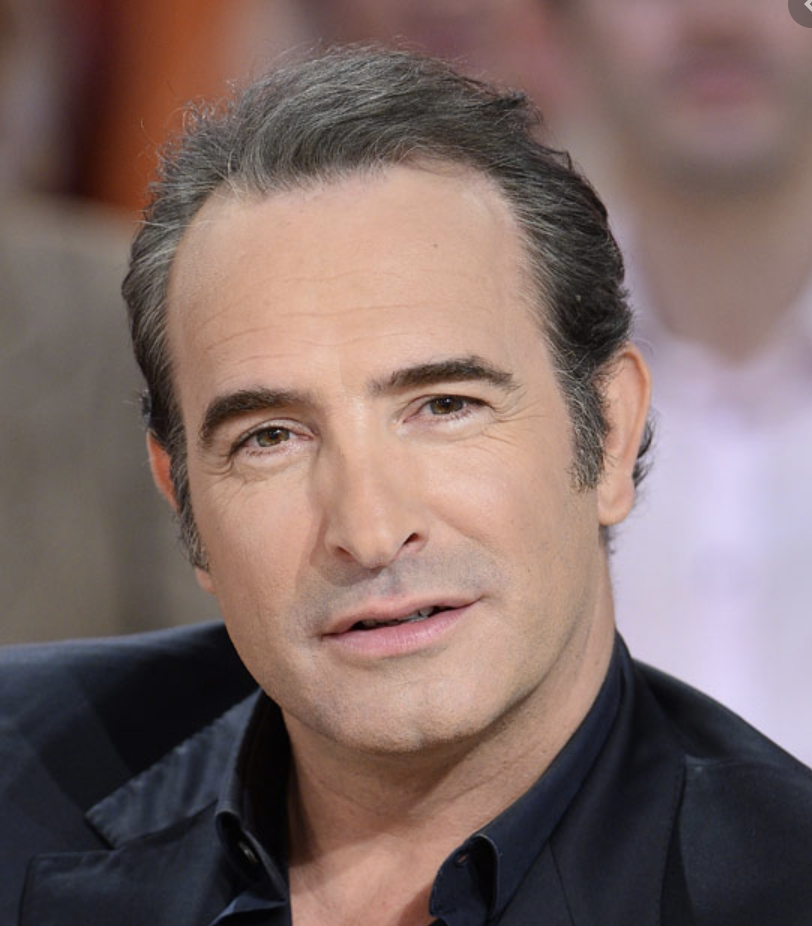
\includegraphics[width=.2\linewidth]{Images/Temporary_pic.png}
\label{fig:cir_example}
\caption{CIR example.}
\end{figure}

The \gls{cir} shown for Fig. \ref{fig:cir_example} has been generated in a rectangular cluttered room of 15 over 10m, filled with furnitures. The selected bandwidth is the same as for the experimental set-up : 499.2MHz. The positions of the tag have been kept the same as in Fig. \ref{fig:cir_ex1}. As one can observe on Fig. \ref{cir}, getting the different peaks is not as trivial.
\vspace{2mm}

From the local maxima  of this \gls{cir}, only the most significant peaks should be extracted, since they likely are associated with the \gls{los} or first reflection. The parameter chosen to reflects the significance of a local maxima is its prominence.
\vspace{2mm}

The algorithm performs a search through the local maxima of the \gls{cir}. First the global maxima is considered as being the first peak corresponding to the \gls{los}. Hence only the local maxima arriving after are considered. Then, the rest of the local maxima are selected from the biggest to the shortest up to the point where $n$ peaks are chosen. All of those peaks are finally sorted based on the time associated with those peaks. 

The algorithm is formalized right beneath :
\vspace{2mm}

\begin{algorithm}[H]
 \KwData{$CIR$ such that $CIR(i)$ is a tuple $[time, val]$, $n \in \mathbb{N}$ the number of peaks requested}
 \KwResult{$Peaks$, ordered list of $n$ tuples.}
Initialization\;
$Peaks(1) \longleftarrow max(CIR)$\;
$CIR \longleftarrow CIR(max:end)$\;
$i \longleftarrow 2$\;
$r \longleftarrow 5$\;
 \While{$i <  n$ and $r < r_{max}$}{	
	\For{$el$ in $CIR$}{
    \If{$el > max(CIR)/r$}{
    $Peaks(i) \longleftarrow el$\;
    $i \longleftarrow i + 1$\;
    }
   }
   $r \longleftarrow r + 1$
 }
 $Order(Peaks)$
 \caption{Peaks Extraction \label{algo:peaks}}
\end{algorithm}

\section{Hard localization algorithm}

This locating system is based on the idea of trilateration and tries to mimic it. Using three peaks, it tries to associate those with the anchor and two virtual anchors to find an intersection point as in the Fig. \ref{fig:triangulation}. Those three peaks are extracted with the algorithm \ref{algo:peaks} from the received \gls{cir} at the tag. As brieftly explained is section \ref{loc_syst_mpc}, there is two main difference with the theoretical case.

\begin{enumerate}
\item The peaks are not associated with a specific anchor
\item Peaks being to close in the infinite bandwidth response could be combined
\end{enumerate}

The first problem has a kind of direct solution, which is trying all the different  of \gls{vas} possible. This is quite straightforward in a simple square or rectangular, since only four \gls{va} exist, leading to six different combinations : $C(4,2) = \frac{4!}{(4-2)!2!} = 6$. Of course, with more complex geometry, the number of permutation to test just keep growing.
\vspace{2mm}

The second problem can be seen on Fig. \ref{fig:inftofin}. Indeed, the two first peaks are in this case too close to each other in time, hence on the right graph, only one peak can be distinguished. 

\begin{figure}[H]
\centering
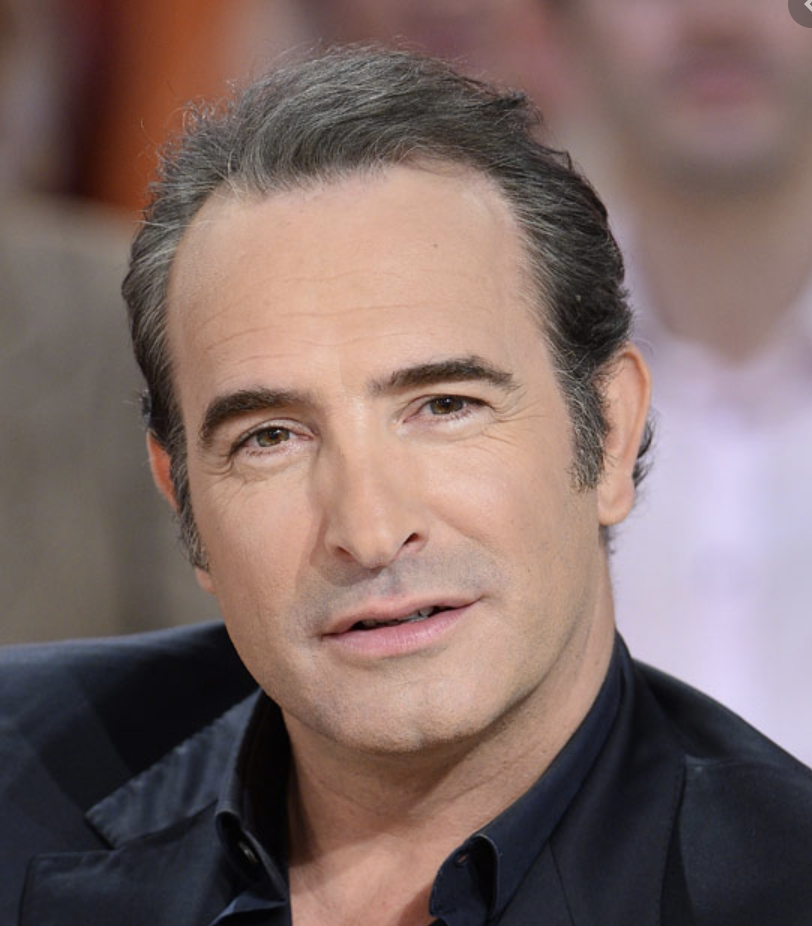
\includegraphics[width=.2\linewidth]{Images/Temporary_pic.png}
\label{fig:inftofin}
\caption{Comparison between an infinite BW CIR and a finite one}
\end{figure}

For each possible combination of anchors, the algorithm will try to solve the system of equations two times. The  \gls{vas} being permuted for each combination since the origin of a specific reflected peak is not known. Based on each of those systems, three different subsystems formed by two out of the three equations are solved for $(x_0, y_0)$. Each of those subsystem is supposed to give 0, 1 or 2 solutions depending on the intersection type between the two circles. The solutions from the three subsystems are regrouped in an array and compared. If three out of the six positions indicates the same area, one can assume that the position as been well retrieved.
\vspace{2mm}

In the cases 

In this case where the two \gls{vas} are selected in the right order, 

- Mettre le schéma de l'antenne qui est dans un coin, et des 4 zones qui se dessinent
	- Ne pas oublier le cas où l'on a 6 zones en fait (dans les pièces rectangulaires)
- Expliquer qu'on va tester toutes les possibilités 2 à 2, mais qu'on peut éliminer certaines avec l'algo speed 2.
- Expliquer que si ça ne marche pas 2à2, on test les cas où les rayons qui arrivent sont confondus.


Les problèmes de cet algo proviennent en partie des symmétries, mais on verra ça dans la simulation, ne pas encore en parler mtn

\section{Soft localization algorithm}

\subsection{CIR MSE}

Pour la forme de la CIR, bien expliquer pourquoi ça ne marche pas vraiment. Même en atténuant les autres pics de la même manière que le pic principal. Parce que la réponse qu'on reçoit peut avoir un LoS légèrement plus obstrué que le reste, ou vice versa. Ca marche bien dans la simulation, mais ça sera probablement moins efficace IRL.

\subsection{Time MSE}

Méthode préférée à CIR

\section{Speed-Up Algorithms}

\subsection{Speed-Up 1}

The aim of this algorithm is to speed up the locating process by reducing the number of needed computations. To achieve this, the \gls{cir}, that needs to be computed at each location, is only computed in a reduced set of possible position for the tag.
\vspace{2mm}

Using the \gls{sdstwr}, the \gls{tof} of the signal between the tag and the anchor can be computed\footnote{In the simulation, it will be assumed to be extracted from the \gls{cir}}. Based on this \gls{tof}, a circle can be traced with the center on this anchor and the radius being the estimated distance deduced from the \gls{tof}. In theory, the tag is supposed to be located on this circle, but due to the discretization and errors on the \gls{tof}, a margin is taken to get the set of possible locations. This margin resides in the two orange circles, that can be observed on Fig. \ref{fig:speedup_1}.
\vspace{2mm}

\begin{figure}[H]
\centering
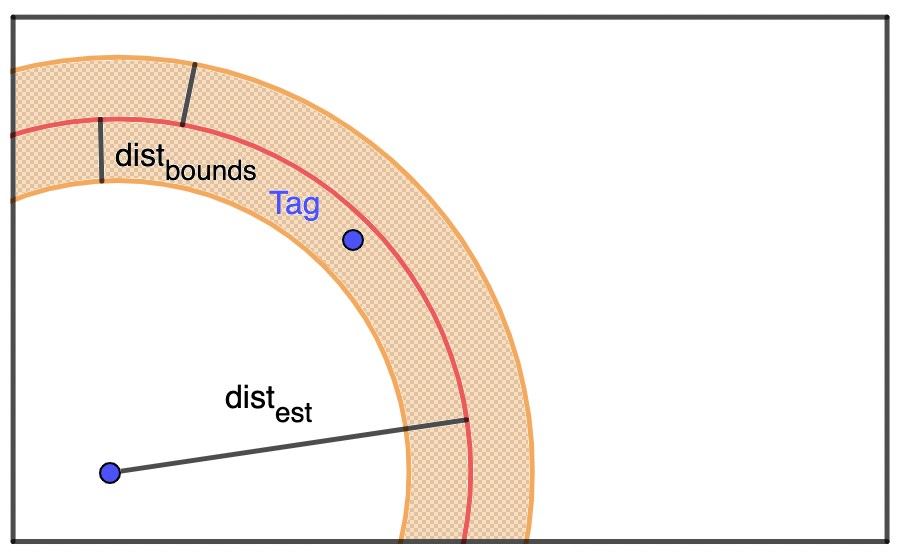
\includegraphics[width=.65\linewidth]{Images/algo_1.png}
\caption{Example of algo 1}
\label{fig:speedup_1}
\end{figure}

From the position inside those boundaries, a mask matrix representing all the position of the room is filled with ones for the position inside of the orange zone. The other positions are left to zero. Later, this mask is used to reduce the computations since only the values associated with a one will be tested.

\subsection{Speed-Up 2}

Choix des ancres en utilsant l'algorithme numéro 1


